\documentclass{article}
\usepackage{xcolor}
\usepackage{titleps}
\usepackage[letterpaper, margin=0.95in]{geometry}
\usepackage{url}
\usepackage{amsmath}
\usepackage{amssymb}
\usepackage{wrapfig}
\usepackage{float}
\usepackage{mathtools}
\usepackage{enumitem}
\usepackage{tabu}
\usepackage{parskip}
\usepackage{natbib}
\usepackage{listings}

\usepackage[many]{tcolorbox}
\usepackage{minted}
\setminted[python]{
	% frame=single,
	% linenos,
    xleftmargin=0.475em,
    baselinestretch=1.2,
}
% https://tex.stackexchange.com/a/569249
\setcounter{secnumdepth}{5}
\setcounter{tocdepth}{5}
\makeatletter
\newcommand\subsubsubsection{\@startsection{paragraph}{4}{\z@}{-2.5ex\@plus -1ex \@minus -.25ex}{1.25ex \@plus .25ex}{\normalfont\normalsize\bfseries}}
\newcommand\subsubsubsubsection{\@startsection{subparagraph}{5}{\z@}{-2.5ex\@plus -1ex \@minus -.25ex}{1.25ex \@plus .25ex}{\normalfont\normalsize\bfseries}}
\makeatother

\usepackage{hyperref}
\usepackage[color=red]{todonotes}
\usepackage{forest}
\definecolor{light-yellow}{HTML}{FFE5CC}

\newpagestyle{ruled}
{\sethead{CMU 16-831}{Introduction to Robot Learning }{Fall 2023}\headrule
  \setfoot{}{}{}}
\pagestyle{ruled}

\renewcommand\makeheadrule{\color{black}\rule[-.75\baselineskip]{\linewidth}{0.4pt}}
\renewcommand*\footnoterule{}

\newtcolorbox[]{answer}[1][]{
    % breakable,
    enhanced,
    nobeforeafter,
    colback=white,
    title=Your Answer,
    sidebyside align=top,
    box align=top,
    #1
}



\begin{document}

\lstset{basicstyle = \ttfamily,columns=fullflexible,
backgroundcolor = \color{light-yellow}
}

\begin{centering}
    {\Large Assignment 2: Policy Gradient} \\
    \vspace{.25cm}
    % \textbf{Due September 13, 11:59 pm} \\
\end{centering}
\vspace{0.25cm}

\textbf{Andrew ID:} \texttt{guangzhl} \\
\textbf{Collaborators:} \texttt{weihaoz}\\ 
\textbf{NOTE:} Please do \textbf{NOT} change the sizes of the answer blocks or plots.

\setcounter{section}{4}
\section{Small-Scale Experiments}

\subsection{Experiment 1 (Cartpole) -- \lbrack25 points total\rbrack}

\subsubsection{Configurations}
\begin{answer}[title=Q5.1.1 with exp1.sh,width=\linewidth]
% TODO
\begin{minted}
[framesep=2mm, fontsize=\scriptsize, breaklines]
{bash}
#!/bin/bash

# Experiment 1: q1_sb_no_rtg_dsa
echo "======================" && \
echo "Running experiment: q1_sb_no_rtg_dsa" && \
echo "Settings: --env_name CartPole-v0 -n 100 -b 1000 -dsa" && \
python rob831/scripts/run_hw2.py --env_name CartPole-v0 -n 100 -b 1000 -dsa --exp_name q1_sb_no_rtg_dsa &

# Experiment 2: q1_sb_rtg_dsa
echo "======================" && \
echo "Running experiment: q1_sb_rtg_dsa" && \
echo "Settings: --env_name CartPole-v0 -n 100 -b 1000 -rtg -dsa" && \
python rob831/scripts/run_hw2.py --env_name CartPole-v0 -n 100 -b 1000 -rtg -dsa --exp_name q1_sb_rtg_dsa &

# Experiment 3: q1_sb_rtg_na
echo "======================" && \
echo "Running experiment: q1_sb_rtg_na" && \
echo "Settings: --env_name CartPole-v0 -n 100 -b 1000 -rtg" && \
python rob831/scripts/run_hw2.py --env_name CartPole-v0 -n 100 -b 1000 -rtg --exp_name q1_sb_rtg_na 

# Experiment 4: q1_lb_no_rtg_dsa
echo "======================" && \
echo "Running experiment: q1_lb_no_rtg_dsa" && \
echo "Settings: --env_name CartPole-v0 -n 100 -b 5000 -dsa" && \
python rob831/scripts/run_hw2.py --env_name CartPole-v0 -n 100 -b 5000 -dsa --exp_name q1_lb_no_rtg_dsa &

# Experiment 5: q1_lb_rtg_dsa
echo "======================" && \
echo "Running experiment: q1_lb_rtg_dsa" && \
echo "Settings: --env_name CartPole-v0 -n 100 -b 5000 -rtg -dsa" && \
python rob831/scripts/run_hw2.py --env_name CartPole-v0 -n 100 -b 5000 -rtg -dsa --exp_name q1_lb_rtg_dsa &

# Experiment 6: q1_lb_rtg_na
echo "======================" && \
echo "Running experiment: q1_lb_rtg_na" && \
echo "Settings: --env_name CartPole-v0 -n 100 -b 5000 -rtg" && \
python rob831/scripts/run_hw2.py --env_name CartPole-v0 -n 100 -b 5000 -rtg --exp_name q1_lb_rtg_na

# echo "======================"
# echo "All experiments completed!"

\end{minted}
\end{answer}

\subsubsection{Plots}

\subsubsubsection{Small batch -- \lbrack5 points\rbrack}
\begin{answer}[title=Q5.1.2.1,height=9.5cm,width=\linewidth]
% TODO
\centering
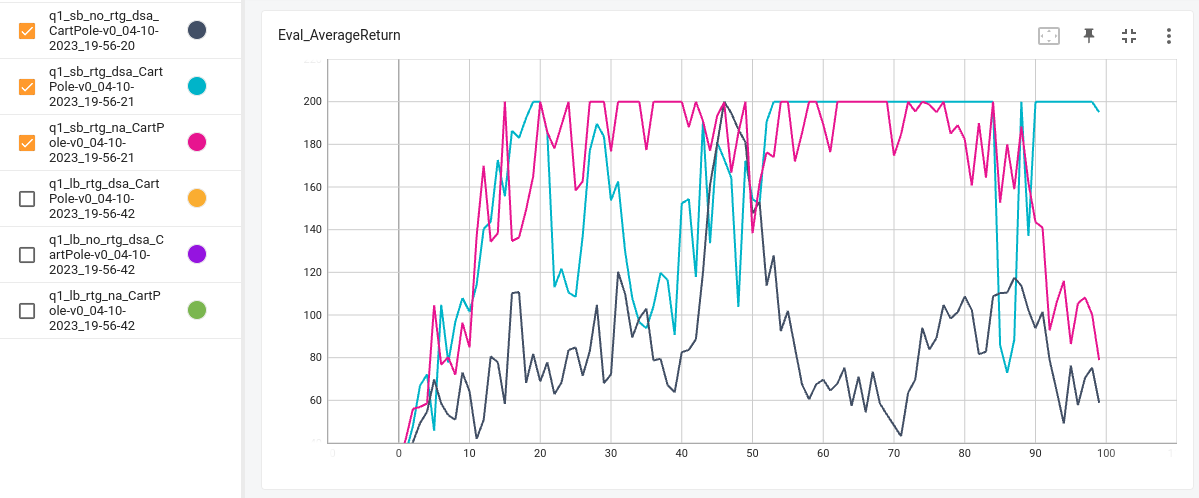
\includegraphics[width=0.9\linewidth]{Images/q1_sb.png}
\end{answer}

\subsubsubsection{Large batch -- \lbrack5 points\rbrack}
\begin{answer}[title=Q5.1.2.2,height=9.5cm,width=\linewidth]
% TODO
\centering
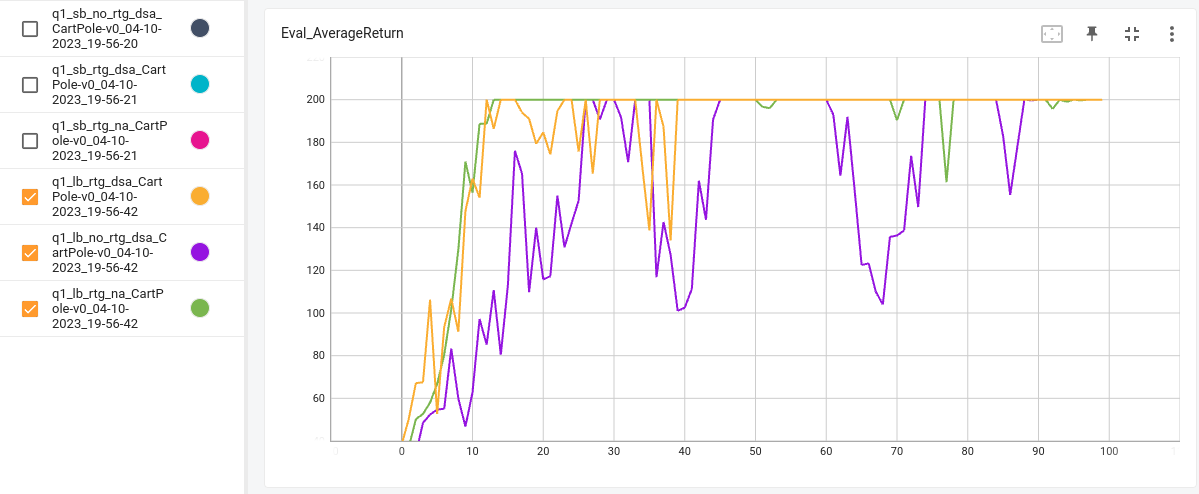
\includegraphics[width=0.9\linewidth]{Images/q1_lb.png}
\end{answer}

\subsubsection{Analysis}

\subsubsubsection{Value estimator -- \lbrack5 points\rbrack}
\begin{answer}[title=Q5.1.3.1,height=4cm,width=\linewidth]
% TODO
The one using reward-to-go is better and produces stabler results because of two reasons. First, reward-to-go makes physical sense to evaluate the subsequent rewards after an action is executed. Second, mathematically, this reduces misguidance/variance for the policy to learn better.

\end{answer}

\subsubsubsection{Advantage standardization -- \lbrack5 points\rbrack}
\begin{answer}[title=Q5.1.3.2,height=4cm,width=\linewidth]
% TODO
The advantage standardization perceivably makes the evaluation average reward stabler and higher compared to other settings.
\end{answer}

\subsubsubsection{Batch size -- \lbrack5 points\rbrack}
\begin{answer}[title=Q5.1.3.1,height=4cm,width=\linewidth]
% TODO
From the result, it is shown that the larger the batch size, the quicker to reach to higher rewards given same amount of iterations.
\end{answer}

\subsection{Experiment 2 (InvertedPendulum) -- \lbrack15 points total\rbrack}

\subsubsection{Configurations -- \lbrack5 points\rbrack}
\begin{answer}[title=Q5.2.1 with exp2.sh,width=\linewidth]
% TODO
\begin{minted}
[framesep=2mm, fontsize=\scriptsize, breaklines]
{bash}
#!/bin/bash

# Define arrays of values you want to try for b* and r*

# Reach training goal of 1000 within 100 iterations but not stablized
# batch_sizes=(900)
# learning_rates=(0.06)

# Approaching to the perform to the "B" level in piazza
batch_sizes=(20000)
learning_rates=(0.01)

# Counter for simultaneous processes
count=0

# Loop over all combinations of batch size and learning rate
for b in "${batch_sizes[@]}"; do
    for r in "${learning_rates[@]}"; do
        # Run the command in the background
        python rob831/scripts/run_hw2.py --env_name InvertedPendulum-v4 \
        --ep_len 1000 --discount 0.9 -n 100 -l 2 -s 64 -b $b -lr $r -rtg \
        --exp_name q2_b${b}_r${r} &

        # Increment the counter
        ((count++))

        # If 3 processes are running, wait for them to finish
        if ((count % 3 == 0)); then
            wait
        fi
    done
done

# Wait for any remaining processes to finish
wait
echo "Experiment 2 is done!"
\end{minted}
\end{answer}

\subsubsection{smallest \textbf{b*} and largest \textbf{r*} (same run) -- \lbrack5 points\rbrack}
\begin{answer}[title=Q5.2.2,height=4cm,width=\linewidth]
% TODO
Reach training goal of 1000 within 100 iterations but not stabilized \\
batch sizes = 900 \\
learning rates= 0.06 
\\
Approaching to the perform to the "B" level in piazza \\
batch sizes = 20000 \\
learning rates = 0.01  \\
\end{answer}

\subsubsection{Plot -- \lbrack5 points\rbrack}
\begin{answer}[title=Q5.2.3,height=10cm,width=\linewidth]
% TODO
\centering
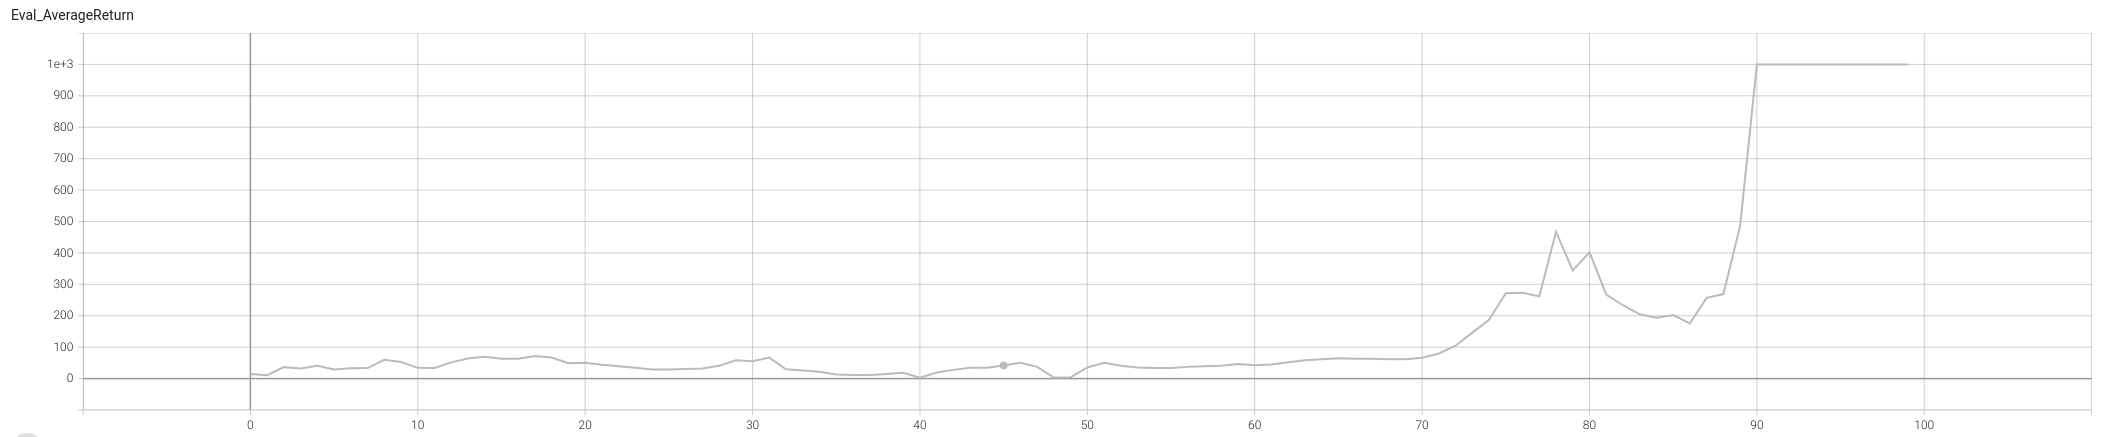
\includegraphics[width=0.9\linewidth]{Images/q2_b900_r0.06.png}
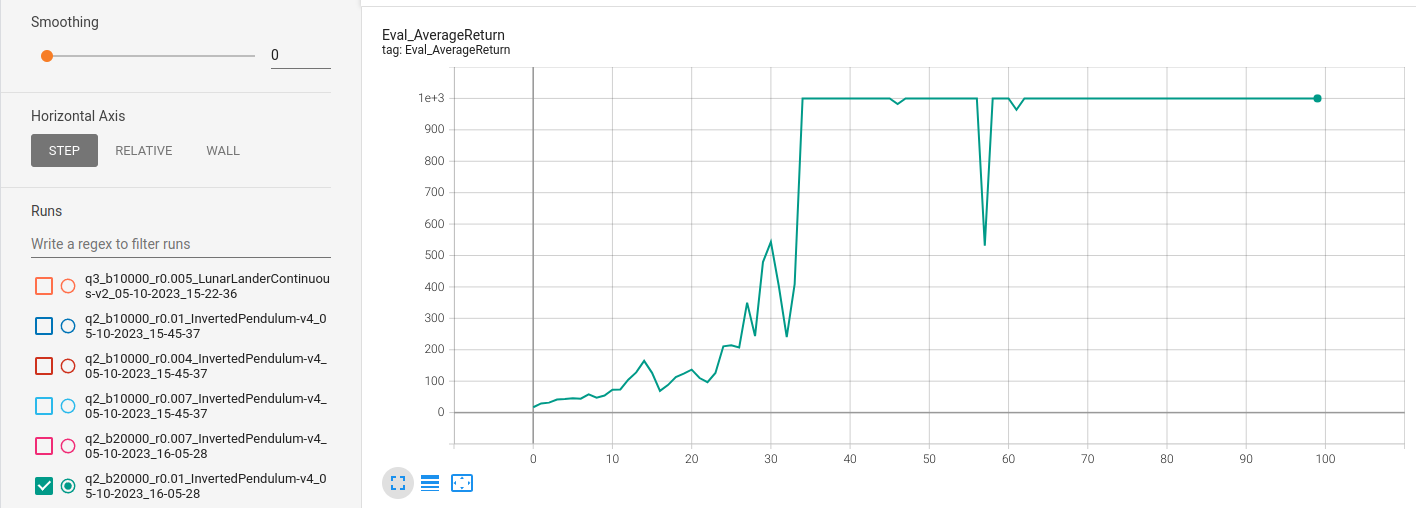
\includegraphics[width=0.9\linewidth]{Images/q2_b20000_r0.01.png}
\end{answer}

\setcounter{section}{6}
\section{More Complex Experiments}

\subsection{Experiment 3 (LunarLander) -- \lbrack10 points total\rbrack}

\subsubsection{Configurations}
\begin{answer}[title=Q7.1.1 with exp3.sh,height=6cm,width=\linewidth]
\begin{minted}
[framesep=2mm, fontsize=\scriptsize, breaklines]
{bash}
python rob831/scripts/run_hw2.py \
    --env_name LunarLanderContinuous-v4 --ep_len 1000
    --discount 0.99 -n 100 -l 2 -s 64 -b 40000 -lr 0.005 \
    --reward_to_go --nn_baseline --exp_name q3_b40000_r0.005
\end{minted}
\end{answer}

\subsubsection{Plot -- \lbrack10 points\rbrack}
\begin{answer}[title=Q7.1.2,height=10cm,width=\linewidth]
% TODO
\centering
\includegraphics[width=0.9\linewidth]{Images/q3_b10000_reward>120.png}
\end{answer}

\subsection{Experiment 4 (HalfCheetah) -- \lbrack30 points\rbrack}

\subsubsection{Configurations}
\begin{answer}[title=Q7.2.1 with exp4.sh,width=\linewidth]
\begin{minted}
[framesep=2mm, fontsize=\scriptsize, breaklines, escapeinside=||, mathescape=true]
{python}
python rob831/scripts/run_hw2.py --env_name HalfCheetah-v4 --ep_len 150 \
--discount 0.95 -n 100 -l 2 -s 32 -b 10000 -lr 0.02 \
--exp_name q4_b10000_r0.02 &

python rob831/scripts/run_hw2.py --env_name HalfCheetah-v4 --ep_len 150 \
--discount 0.95 -n 100 -l 2 -s 32 -b 10000 -lr 0.02 -rtg \
--exp_name q4_b10000_r0.02_rtg

python rob831/scripts/run_hw2.py --env_name HalfCheetah-v4 --ep_len 150 \
--discount 0.95 -n 100 -l 2 -s 32 -b 10000 -lr 0.02 --nn_baseline \
--exp_name q4_b10000_r0.02_nnbaseline &

python rob831/scripts/run_hw2.py --env_name HalfCheetah-v4 --ep_len 150 \
--discount 0.95 -n 100 -l 2 -s 32 -b 10000 -lr 0.02 -rtg --nn_baseline \
--exp_name q4_b10000_r0.02_rtg_nnbaseline 
\end{minted}
\end{answer}

\subsubsection{Plot -- \lbrack10 points\rbrack}
\begin{answer}[title=Q7.2.2 with exp4.sh,height=10cm,width=\linewidth]
% TODO
\centering
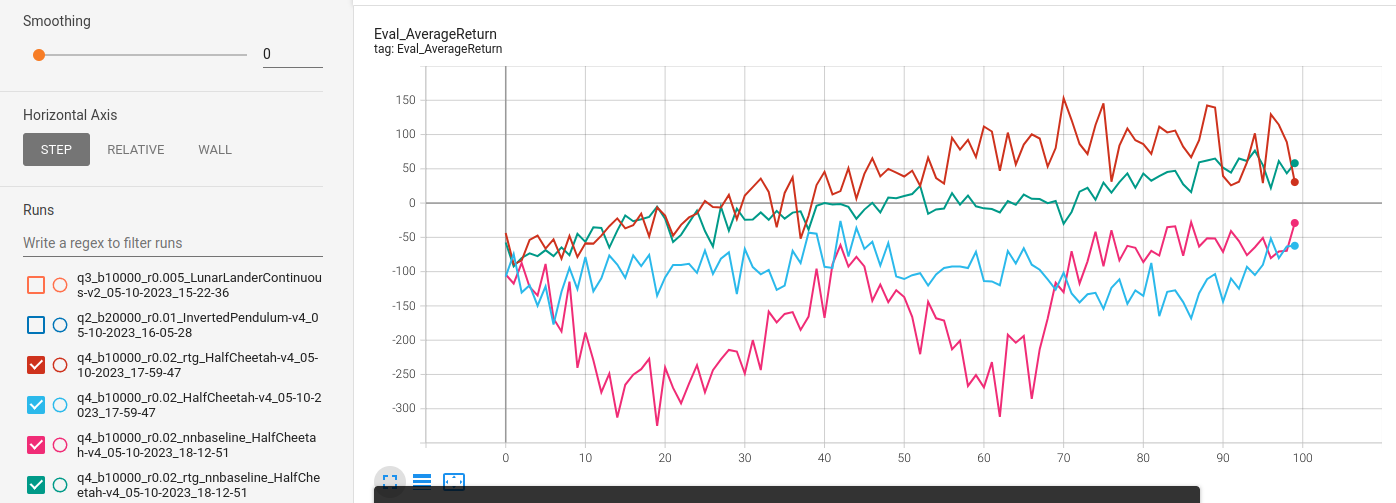
\includegraphics[width=0.9\linewidth]{Images/q4_b10000_r0.02.png}
As instructed on piazza, the average return of the best setup is bigger than 50.
\end{answer}



\subsubsection{Optimal b* and r* -- \lbrack3 points\rbrack}
\begin{answer}[title=Q7.2.3,height=4cm,width=\linewidth]
% TODO
This linear search for optimal parameters are skipped per instructions on piazza.
\end{answer}

\subsubsection{Describe how b* and r* affect task performance -- \lbrack7 points\rbrack}
\begin{answer}[title=Q7.2.4,height=4cm,width=\linewidth]
% TODO
In general the bigger the batch size, the better training performance per iteration. However, for learning rate, if it is too small, the policy learns really slow; if it is too big, the training would become unstable and resulting policy would have undefined behavior.
\end{answer}

\subsubsection{Configurations with optimal b* and r* -- \lbrack3 points\rbrack}
\begin{answer}[title=Q7.2.5 with exp5.sh,height=6cm,width=\linewidth]
% TODO
\begin{minted}
[framesep=2mm, fontsize=\scriptsize, breaklines]
{bash}
python rob831/scripts/run_hw2.py --env_name HalfCheetah-v4 --ep_len 150 \
    --discount 0.95 -n 100 -l 2 -s 32 -b <b*> -lr <r*> \
    --exp_name q4_b<b*>_r<r*>

python rob831/scripts/run_hw2.py --env_name HalfCheetah-v4 --ep_len 150 \
    --discount 0.95 -n 100 -l 2 -s 32 -b <b*> -lr <r*> -rtg \
    --exp_name q4_b<b*>_r<r*>_rtg

python rob831/scripts/run_hw2.py --env_name HalfCheetah-v4 --ep_len 150 \
    --discount 0.95 -n 100 -l 2 -s 32 -b <b*> -lr <r*> --nn_baseline \
    --exp_name q4_b<b*>_r<r*>_nnbaseline

python rob831/scripts/run_hw2.py --env_name HalfCheetah-v4 --ep_len 150 \
    --discount 0.95 -n 100 -l 2 -s 32 -b <b*> -lr <r*> -rtg --nn_baseline \
    --exp_name q4_b<b*>_r<r*>_rtg_nnbaseline
\end{minted}
\end{answer}

\subsubsection{Plot for four runs with optimal b* and r* -- \lbrack7 points\rbrack}
\begin{answer}[title=Q7.2.6,height=10cm,width=\linewidth]
% TODO
\centering
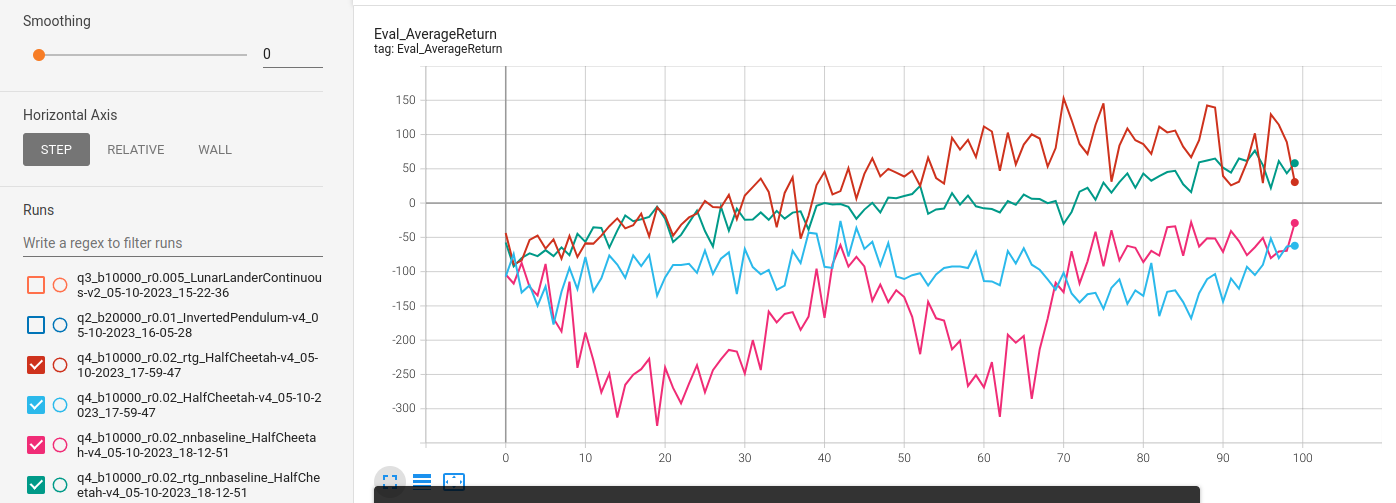
\includegraphics[width=0.9\linewidth]{Images/q4_b10000_r0.02.png}

As instructed on piazza, the average return of the best setup is bigger than 50.
\end{answer}


\section{Implementing Generalized Advantage Estimation}

\subsection{Experiment 5 (Hopper) -- \lbrack20 points\rbrack}

\subsubsection{Configurations}
\begin{answer}[title=Q8.1.1 with exp5.sh,width=\linewidth]
\begin{minted}
[framesep=2mm, fontsize=\scriptsize, breaklines, escapeinside=||, mathescape=true]
{python}
#!/bin/bash

# Define the lambda values
lambdas=(0 0.95 0.99 1)

# Counter for simultaneous processes
count=0

# Loop over all lambda values
for lambda in "${lambdas[@]}"; do
    # Run the command in the background
    python rob831/scripts/run_hw2.py \
    --env_name Hopper-v4 --ep_len 1000 \
    --discount 0.99 -n 300 -l 2 -s 32 -b 2000 -lr 0.001 \
    --reward_to_go --nn_baseline --action_noise_std 0.5 --gae_lambda $lambda \
    --exp_name q5_b2000_r0.001_lambda$lambda &

    # Increment the counter
    ((count++))

    # If 3 processes are running, wait for them to finish
    if ((count % 3 == 0)); then
        wait
    fi
done

# Wait for any remaining processes to finish
wait
echo "Experiment 5 is done!"
\end{minted}
\end{answer}

\subsubsection{Plot -- \lbrack13 points\rbrack}
\begin{answer}[title=Q8.1.2,height=10cm,width=\linewidth]
% TODO
\centering
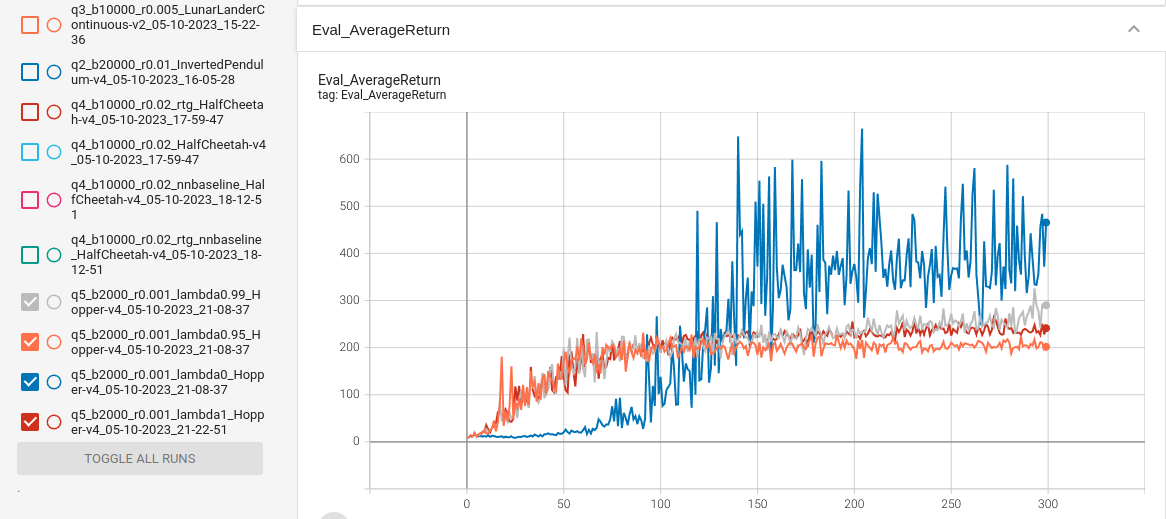
\includegraphics[width=0.9\linewidth]{Images/q5.png}
\end{answer}

\subsubsection{Describe how $\lambda$ affects task performance -- \lbrack7 points\rbrack}
\begin{answer}[title=Q8.1.3,height=6cm,width=\linewidth]
% TODO
From the result, when ${\lambda}$ is 1 or 0.99 or 0.95, they are or at least very close to the vanilla neural network baseline estimator with summation of the discounted trajectory rewards upfront. This possesses less bias but introduces strong variance in the data collected. On the other hand, when ${\lambda}$ is 0, the advantage at each step is the temporal difference where the upcoming reward is obtained from a value function. This has low variance but high bias. In the training evaluation result, it is somewhat explainable with the aforementioned: the temporal difference end of the spectrum has huge variance while the others are a lot stabler; the state-dependent value function learns slowly due to an initial lack of data but is able to enable the temporal difference setup (${\lambda}$=0) to have better average return after learned a decent mapping from state to future returns.
\end{answer}

\clearpage

\section{Bonus! (optional)}

\subsection{Parallelization -- \lbrack15 points\rbrack}
\begin{answer}[title=Q9.1 not finished but with some progress!!!,width=\linewidth]
% TODO (optional)
Difference in training time: 
\vspace{1.0cm}
\begin{minted}
[framesep=2mm, fontsize=\scriptsize, breaklines]
{python}
    def worker(self, start, end, collect_policy, eval_policy, initial_expertdata, relabel_with_expert, start_relabel_with_expert, expert_policy, total_envsteps):
        for itr in range(start, end):
            print("\n\n********** Iteration %i ************"%itr)

            # decide if videos should be rendered/logged at this iteration
            if itr % self.params['video_log_freq'] == 0 and self.params['video_log_freq'] != -1:
                self.log_video = True
            else:
                self.log_video = False

            # decide if metrics should be logged
            if self.params['scalar_log_freq'] == -1:
                self.log_metrics = False
            elif itr % self.params['scalar_log_freq'] == 0:
                self.log_metrics = True
            else:
                self.log_metrics = False

            # collect trajectories, to be used for training
            training_returns = self.collect_training_trajectories(itr,
                                initial_expertdata, collect_policy,
                                self.params['batch_size'])
            paths, envsteps_this_batch, train_video_paths = training_returns
            with total_envsteps.get_lock():
                total_envsteps.value += envsteps_this_batch

            # add collected data to replay buffer
            self.agent.add_to_replay_buffer(paths)

            # train agent (using sampled data from replay buffer)
            train_logs = self.train_agent()

            # log/save
            if self.log_video or self.log_metrics:
                # perform logging
                print('\nBeginning logging procedure...')
                self.perform_logging(itr, paths, eval_policy, train_video_paths, train_logs)

                if self.params['save_params']:
                    self.agent.save('{}/agent_itr_{}.pt'.format(self.params['logdir'], itr))
\end{minted}
\end{answer}

\begin{answer}[title=Q9.1 conti' not finished but with some progress!!!,width=\linewidth]
% TODO (optional)
Difference in training time: 
\vspace{1.0cm}
\begin{minted}
[framesep=2mm, fontsize=\scriptsize, breaklines]
{python}
    def run_training_loop(self, n_iter, collect_policy, eval_policy, initial_expertdata=None, relabel_with_expert=False, start_relabel_with_expert=1, expert_policy=None):
        """
        :param n_iter:  number of (dagger) iterations
        :param collect_policy:
        :param eval_policy:
        :param initial_expertdata:
        :param relabel_with_expert:  whether to perform dagger
        :param start_relabel_with_expert: iteration at which to start relabel with expert
        :param expert_policy:
        """

        # init vars at beginning of training
        self.total_envsteps = mp.Value('i', 0, lock=True)  # multiprocessing Value to share data across processes
        self.start_time = time.time()

        # Number of workers (logical cores)
        num_workers = mp.cpu_count()

        # Split iterations across workers
        iter_per_worker = n_iter // num_workers

        processes = []
        for i in range(num_workers):
            start_iter = i * iter_per_worker
            end_iter = (i + 1) * iter_per_worker if i != num_workers - 1 else n_iter

            p = mp.Process(target=self.worker, args=(start_iter, end_iter, collect_policy, eval_policy, initial_expertdata, relabel_with_expert, start_relabel_with_expert, expert_policy, self.total_envsteps))
            p.start()
            processes.append(p)

        for p in processes:
            p.join()
 
        self.total_envsteps = self.total_envsteps.value  # Convert back to regular int after all processes have finished

\end{minted}
\end{answer}

\subsection{Multiple gradient steps -- \lbrack5 points\rbrack}
\begin{answer}[title=Q9.1,height=14cm,width=\linewidth]
% TODO (optional)
\centering
\includegraphics[height=8cm]{example-image-a}

\vspace{1.0cm}
\begin{minted}
[framesep=2mm, fontsize=\scriptsize, breaklines]
{bash}
python rob831/scripts/run_hw2.py \
\end{minted}

\end{answer}

\end{document}

